% vim: set textwidth=120:

% Example CV based on the 1.5-column-cv template. Main features:
% * uses the Roboto font family and IcoMoon icon set;
% * doesn't use colours, different font weights are used instead for styling;
% * because the CV fits on one page, header and footer is empty, since there isn't much useful info to put there;
% * includes a photo.
\documentclass[a4paper,10pt]{article}


% package imports
% ---------------

\usepackage[british]{babel} % for correct language and hyphenation and stuff
\usepackage{calc}           % for easier length calculations (infix notation)
\usepackage{enumitem}       % for configuring list environments
\usepackage{fancyhdr}       % for setting header and footer
\usepackage{fontspec}       % for fonts
\usepackage{geometry}       % for setting margins (\newgeometry)
\usepackage{graphicx}       % for pictures
\usepackage{microtype}      % for microtypography stuff
\usepackage{xcolor}         % for colours


% margin and column widths
% ------------------------

% margins
\newgeometry{left=15mm,right=15mm,top=15mm,bottom=15mm}

% width of the gap between left and right column
\newlength{\cvcolumngapwidth}
\setlength{\cvcolumngapwidth}{3.5mm}

% left column width
\newlength{\cvleftcolumnwidth}
\setlength{\cvleftcolumnwidth}{44.5mm}

% right column width
\newlength{\cvrightcolumnwidth}
\setlength{\cvrightcolumnwidth}{\textwidth-\cvleftcolumnwidth-\cvcolumngapwidth}

% set paragraph indentation to 0, because it screws up the whole layout otherwise
\setlength{\parindent}{0mm}


% style definitions
% -----------------
% style categories explanation:
% * \cvnameXXX is used for the name;
% * \cvsectionXXX is used for section names (left column, accompanied by a horizontal rule);
% * \cvtitleXXX is used for job/education titles (right column);
% * \cvdurationXXX is used for job/education durations (left column);
% * \cvheadingXXX is used for headings (left column);
% * \cvmainXXX (and \setmainfont) is used for main text;
% * \cvruleXXX is used for the horizontal rules denoting sections.

% font families
\defaultfontfeatures{Ligatures=TeX} % reportedly a good idea, see https://tex.stackexchange.com/a/37251

\newfontfamily{\cvnamefont}[Path=resources/Roboto/]{Roboto-Medium.ttf}
\newfontfamily{\cvsectionfont}[Path=resources/Roboto/]{Roboto-Medium.ttf}
\newfontfamily{\cvtitlefont}[Path=resources/Roboto/]{Roboto-Regular.ttf}
\newfontfamily{\cvdurationfont}[Path=resources/Roboto/]{Roboto-LightItalic.ttf}
\newfontfamily{\cvheadingfont}[Path=resources/Roboto/]{Roboto-Regular.ttf}
\setmainfont[Path=resources/Roboto/]{Roboto-Light.ttf}

% colours
\definecolor{cvnamecolor}{HTML}{000000}
\definecolor{cvsectioncolor}{HTML}{000000}
\definecolor{cvtitlecolor}{HTML}{000000}
\definecolor{cvdurationcolor}{HTML}{000000}
\definecolor{cvheadingcolor}{HTML}{000000}
\definecolor{cvmaincolor}{HTML}{000000}
\definecolor{cvrulecolor}{HTML}{000000}

\color{cvmaincolor}

% styles
\newcommand{\cvnamestyle}[1]{{\Large\cvnamefont\textcolor{cvnamecolor}{#1}}}
\newcommand{\cvsectionstyle}[1]{{\normalsize\cvsectionfont\textcolor{cvsectioncolor}{#1}}}
\newcommand{\cvtitlestyle}[1]{{\large\cvtitlefont\textcolor{cvtitlecolor}{#1}}}
\newcommand{\cvdurationstyle}[1]{{\small\cvdurationfont\textcolor{cvdurationcolor}{#1}}}
\newcommand{\cvheadingstyle}[1]{{\normalsize\cvheadingfont\textcolor{cvheadingcolor}{#1}}}


% inter-item spacing
% ------------------

% vertical space after personal info and standard CV items
\newlength{\cvafteritemskipamount}
\setlength{\cvafteritemskipamount}{5mm plus 1.25mm minus 1.25mm}

% vertical space after sections
\newlength{\cvaftersectionskipamount}
\setlength{\cvaftersectionskipamount}{2mm plus 0.5mm minus 0.5mm}

% extra vertical space to be used when a section starts with an item with a heading (e.g. in the skills section),
% so that the heading does not follow the section name too closely
\newlength{\cvbetweensectionandheadingextraskipamount}
\setlength{\cvbetweensectionandheadingextraskipamount}{1mm plus 0.25mm minus 0.25mm}


% intra-item spacing
% ------------------

% vertical space after name
\newlength{\cvafternameskipamount}
\setlength{\cvafternameskipamount}{3mm plus 0.75mm minus 0.75mm}

% vertical space after personal info lines
\newlength{\cvafterpersonalinfolineskipamount}
\setlength{\cvafterpersonalinfolineskipamount}{2mm plus 0.5mm minus 0.5mm}

% vertical space after titles
\newlength{\cvaftertitleskipamount}
\setlength{\cvaftertitleskipamount}{1mm plus 0.25mm minus 0.25mm}

% value to be used as parskip in right column of CV items and itemsep in lists (same for both, for consistency)
\newlength{\cvparskip}
\setlength{\cvparskip}{0.5mm plus 0.125mm minus 0.125mm}

% set global list configuration (use parskip as itemsep, and no separation otherwise)
\setlist{parsep=0mm,topsep=0mm,partopsep=0mm,itemsep=\cvparskip}


% CV commands
% -----------

% creates a "personal info" CV item with the given left and right column contents, with appropriate vertical space after
% @param #1 left column content (should be the CV photo)
% @param #2 right column content (should be the name and personal info)
\newcommand{\cvpersonalinfo}[2]{
    % left and right column
    \begin{minipage}[t]{\cvleftcolumnwidth}
        \vspace{0mm} % XXX hack to align to top, see https://tex.stackexchange.com/a/11632
        \raggedleft #1
    \end{minipage}% XXX necessary comment to avoid unwanted space
    \hspace{\cvcolumngapwidth}% XXX necessary comment to avoid unwanted space
    \begin{minipage}[t]{\cvrightcolumnwidth}
        \vspace{0mm} % XXX hack to align to top, see https://tex.stackexchange.com/a/11632
        #2
    \end{minipage}

    % space after
    \vspace{\cvafteritemskipamount}
}

% typesets a name, with appropriate vertical space after
% @param #1 name text
\newcommand{\cvname}[1]{
    % name
    \cvnamestyle{#1}

    % space after
    \vspace{\cvafternameskipamount}
}

% typesets a line of personal info beginning with an icon, with appropriate vertical space after
% @param #1 parameters for the \includegraphics command used to include the icon
% @param #2 icon filename
% @param #3 line text
\newcommand{\cvpersonalinfolinewithicon}[3]{
    % icon, vertically aligned with text (see https://tex.stackexchange.com/a/129463)
    \raisebox{.5\fontcharht\font`E-.5\height}{\includegraphics[#1]{#2}}
    % text
    #3

    % space after
    \vspace{\cvafterpersonalinfolineskipamount}
}

% creates a "section" CV item with the given left column content, a horizontal rule in the right column, and with
% appropriate vertical space after
% @param #1 left column content (should be the section name)
\newcommand{\cvsection}[1]{
    % left and right column
    \begin{minipage}[t]{\cvleftcolumnwidth}
        \raggedleft\cvsectionstyle{#1}
    \end{minipage}% XXX necessary comment to avoid unwanted space
    \hspace{\cvcolumngapwidth}% XXX necessary comment to avoid unwanted space
    \begin{minipage}[t]{\cvrightcolumnwidth}
        \textcolor{cvrulecolor}{\rule{\cvrightcolumnwidth}{0.3mm}}
    \end{minipage}

    % space after
    \vspace{\cvaftersectionskipamount}
}

% creates a standard, multi-purpose CV item with the given left and right column contents, parskip set to cvparskip
% in the right column, and with appropriate vertical space after
% @param #1 left column content
% @param #2 right column content
\newcommand{\cvitem}[2]{
    % left and right column
    \begin{minipage}[t]{\cvleftcolumnwidth}
        \raggedleft #1
    \end{minipage}% XXX necessary comment to avoid unwanted space
    \hspace{\cvcolumngapwidth}% XXX necessary comment to avoid unwanted space
    \begin{minipage}[t]{\cvrightcolumnwidth}
        \setlength{\parskip}{\cvparskip} #2
    \end{minipage}

    % space after
    \vspace{\cvafteritemskipamount}
}

% typesets a title, with appropriate vertical space after
% @param #1 title text
\newcommand{\cvtitle}[1]{
    % title
    \cvtitlestyle{#1}

    % space after
    \vspace{\cvaftertitleskipamount}
    % XXX need to subtract cvparskip here, because it is automatically inserted after the title "paragraph"
    \vspace{-\cvparskip}
}


% header and footer
% -----------------

% set empty header and footer
\pagestyle{empty}



% preamble end/document start
% ===========================

\begin{document}


% personal info
% -------------

\cvpersonalinfo{
    % photo
    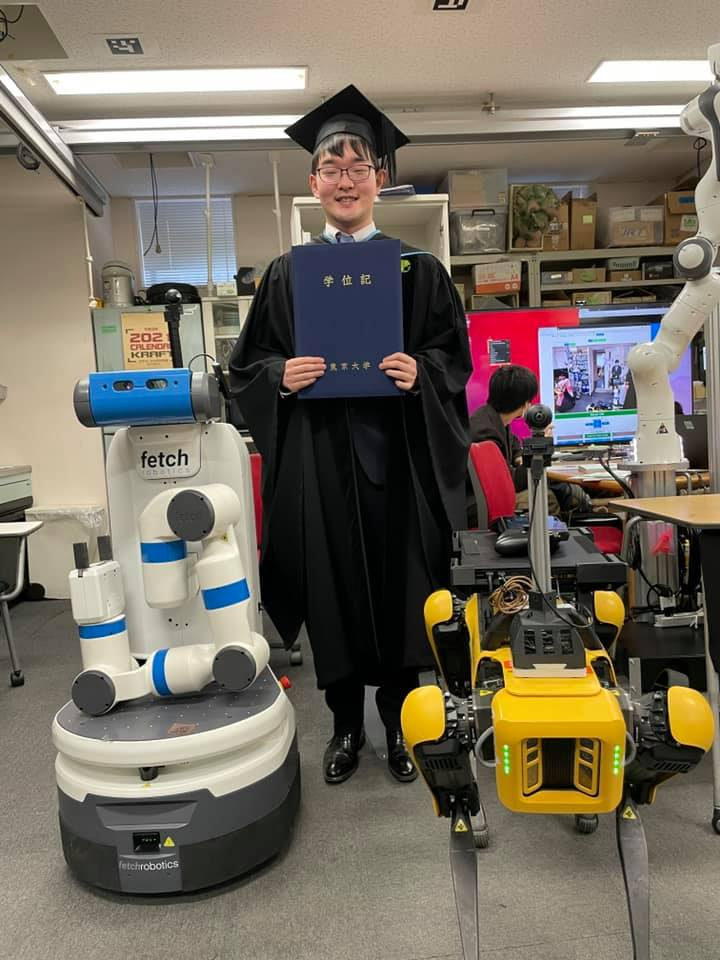
\includegraphics[height=36mm]{resources/photo.jpg}
}{
    % name
    \cvname{Yoshiki Obinata}

    % address
    \cvpersonalinfolinewithicon{height=4mm}{resources/IcoMoon-Free-PDF/072-location.pdf}{
        Tokyo, Japan
    }

    % phone number
    \cvpersonalinfolinewithicon{height=4mm}{resources/IcoMoon-Free-PDF/067-phone.pdf}{
        (Please ask me by e-mail.)
    }

    % email address
    \cvpersonalinfolinewithicon{height=4mm}{resources/IcoMoon-Free-PDF/070-envelop.pdf}{
        obinata (at) jsk.imi.i.u-tokyo.ac.jp
    }

    % LinkedIn account
    \cvpersonalinfolinewithicon{height=4mm}{resources/IcoMoon-Free-PDF/458-linkedin.pdf}{
        yoshikiobinata
    }

    % GitHub account
    \cvpersonalinfolinewithicon{height=4mm}{resources/IcoMoon-Free-PDF/433-github.pdf}{
        https://github.com/mqcmd196
    }

    % date of birth
    Born 3 April 1998
}


% work experience
% ---------------

\cvsection{WORK EXPERIENCE}

\cvitem{
  \cvdurationstyle{April 2025 -- present}
}{
  \cvtitle{Research Fellowship}

  JSPS Research Fellowships for young students (DC2)

  \begin{itemize}[leftmargin=*]
  \item Research Grant 200000 JPY / month
  \item Research Fund 800000 JPY / year
  \end{itemize}
}

\cvitem{
  \cvdurationstyle{July 2023 -- March 2025}
}{
  \cvtitle{Software Engineer / Parttime}

  New Innovations Inc.

  \begin{itemize}[leftmargin=*]
  \item Robotics software engineer
  \item Embedded software engineer
  \end{itemize}
}

\cvitem{
  \cvdurationstyle{April 2023 -- March 2025}
}{
  \cvtitle{The project member of Support for Pioneering Research Initiated by the Next Generation (SPRING)}

  Japan Science and Technology Agency (JST)

  \begin{itemize}[leftmargin=*]
  \item Research Grant 180000 JPY / month
  \item Research Fund 340000 JPY / year
  \end{itemize}
}

\cvitem{
  \cvdurationstyle{May 2021 -- present}
}{
  \cvtitle{Technical Assistant Staff / Parttime}

  JSK Robotics Lab, The University of Tokyo

  \begin{itemize}[leftmargin=*]
    \item Developing and maintaining the robot software.
  \end{itemize}
}

\cvitem{
  \cvdurationstyle{April 2022 -- June 2023}
}{
  \cvtitle{Robotics Software Engineer, Integrator / Parttime}

  Preferred Robotics

  \begin{itemize}[leftmargin=*]
    \item Developing the B2B mobile robot service.
  \end{itemize}
}

\cvitem{
  \cvdurationstyle{August 2017 -- June 2022}
}{
  \cvtitle{Software Engineer / Parttime}

  Aidemy

  \begin{itemize}[leftmargin=*]
    \item Developing the education service of machine-learning-programming.
  \end{itemize}
}

\cvitem{
  \cvdurationstyle{August 2021 -- October 2021}
}{
  \cvtitle{Robotics Software Engineer / Internship}

  Mujin, Inc.

  \begin{itemize}[leftmargin=*]
    \item Developing the robot software.
  \end{itemize}
}

\cvitem{
  \cvdurationstyle{December 2018 -- June 2019}
}{
  \cvtitle{Software Engineer / Internship}
  OTOKORO.com
  \begin{itemize}[leftmargin=*]
    \item Developing of an automated data analysys platform.
  \end{itemize}
}


% education
% ---------

\cvsection{EDUCATION}

% doctor's
\cvitem{
    \cvdurationstyle{2023 -- present}
}{
    \cvtitle{Ph.D's degree in Information Science and Technology}

    Graduate School of Information Science and Technology, The University of Tokyo

    \begin{itemize}[leftmargin=*]
        \item Major in Mechano-Informatics
        \item Belong to JSK Robotics Lab and supervised by Prof.Kei Okada
    \end{itemize}
}

% master's
\cvitem{
    \cvdurationstyle{2021 -- 2023}
}{
    \cvtitle{Master's degree in Information Science and Technology}

    Graduate School of Information Science and Technology, The University of Tokyo

    \begin{itemize}[leftmargin=*]
        \item Major in Mechano-Informatics
        \item Belong to JSK Robotics Lab and supervised by Prof.Kei Okada
    \end{itemize}
}

% bachelor's
\cvitem{
    \cvdurationstyle{2017 -- 2021}
}{
    \cvtitle{Bachelor's degree in Engineering}

    Faculty of Engineering, The University of Tokyo

    \begin{itemize}[leftmargin=*]
        \item Department of Mechano-Informatics
        \item Belong to JSK Robotics Lab and supervised by Prof.Kei Okada
    \end{itemize}
}

% scholarships
% ---------

\cvsection{SCHOLARSHIPS}

\cvitem{
    \cvdurationstyle{2025 -- present}
}{
    \cvtitle{Scholarship}

    Iwadare Scholarship Foundation

    \begin{itemize}[leftmargin=*]
        \item 550000 yen/year for 1 year.
    \end{itemize}
}

\cvitem{
    \cvdurationstyle{2017 -- present}
}{
    \cvtitle{Exemption of tuition fees}

    The University of Tokyo

    \begin{itemize}[leftmargin=*]
        \item Tuition exemption from undergraduate to graduate school
    \end{itemize}
}

\cvitem{
    \cvdurationstyle{2021 -- 2023}
}{
    \cvtitle{Scholarship}

    COSINA Scholarship

    \begin{itemize}[leftmargin=*]
        \item 30000 yen/month for 2 years.
    \end{itemize}
}

\cvitem{
    \cvdurationstyle{2021 -- 2023}
}{
    \cvtitle{Scholarship}

    TAKEUCHI Scholarship

    \begin{itemize}[leftmargin=*]
        \item 60000 yen/month for 2 years.
    \end{itemize}
}


\cvitem{
    \cvdurationstyle{2017 -- 2021}
}{
  \cvtitle{Scholarship}

  The foundation Matsuo Scholarship Society

  \begin{itemize}[leftmargin=*]
  \item Scholarship for school expenses, tuition, dormitory, food, and medical expenses for 4 years.
  \end{itemize}
}


% skills
% ------

\cvsection{SKILLS}

\vspace{\cvbetweensectionandheadingextraskipamount}

% languages
\cvitem{
    \cvheadingstyle{Languages}
}{
  Japanese, English, Chinese
}

% skills
\cvitem{
    \cvheadingstyle{Software Skills}
}{
  Programming Languages
  \begin{itemize}
    \item Python, Lisp, C++, Shell, JavaScript
  \end{itemize}
  Frameworks, Middlewares
  \begin{itemize}
    \item ROS1 / ROS2, OpenCV, Qt, Universal Windows Platform, Active Directory, LDAP
  \end{itemize}
  Operating System
  \begin{itemize}
    \item Linux(Ubuntu, Debian, Red Hat Enterprise Linux), Windows 11, Windows Server, macOS
  \end{itemize}
}


% publications

\cvsection{SELECTED ACHIEVEMENTS}

\vspace{\cvbetweensectionandheadingextraskipamount}

\cvitem{
  \cvheadingstyle{Awards}
}{
  \begin{enumerate}
  \item Kento Kawaharazuka, \underline{Yoshiki Obinata}, Naoaki Kanazawa, Naoto Tsukamoto, Kei Okada. ``Reflexive Open-Vocabulary Navigation without Prior Knowledge Using Omnidirectional Camera and Multiple Vision-Language Models'', Excellent Practice Award (Workshop on Environment Dynamics Matters: Embodied Navigation to Movable Objects) in IROS2024.
  \item \underline{Yoshiki Obinata}, Iori Yanokura, Naoto Tsukamoto, Naoya Yamaguchi, Shingo Kitagawa, Koki Shinjo, Kei Okada, Masayuki Inaba. ``System for Teaching Robot Action Instructions and Responding to Situations Using a Chat Application'', IAS-18 Finalist for the Best Paper Award.
  \item \underline{Yoshiki Obinata}, Kento Kawaharazuka, Naoaki Kanazawa, Naoya Yamaguchi, Naoto Tsukamoto, Iori Yanokura, Shingo Kitagawa, Koki Shinjo, Kei Okada, Masayuki Inaba. Semantic Scene Difference Detection in Daily Life Patroling by Mobile Robots using Pre-Trained Large-Scale Vision-Language Model, IEEE RAS Japan Joint Chapter Young Award (IROS 2023).
  \item \underline{Yoshiki Obinata}, Kento Kawaharazuka, Naoaki Kanazawa, Naoya Yamaguchi, Naoto Tsukamoto, Iori Yanokura, Shingo Kitagawa, Koki Shinjo, Kei Okada, Masayuki Inaba. ``Semantic Scene Difference Detection in Daily Life Patroling by Mobile Robots using Pre-Trained Large-Scale Vision-Language Model'', SICE International Young Authors Award (SIYA-IROS 2023).
  \item \underline{Yoshiki Obinata}, Naoaki Kanazawa, Kento Kawaharazuka, Iori Yanokura, Soonhyo Kim. \newblock {RoboCup@home Japan 2022 General Purpose Service Robot First Prize}.
  \end{enumerate}
}
\cvitem{
  \cvheadingstyle{Journals}
}{
  \begin{enumerate}
  \item \underline{Yoshiki Obinata}, Kento Kawaharazuka, Naoaki Kanazawa, Naoya Yamaguchi, Iori Yanokura, Shingo Kitagawa, Kei Okada, Masayuki Inaba. ``Situation classification of living environment by daily life support robot using pre-trained large-scale vision-language model'', Advanced Robotics, Vol.39, No.7, pp.323--337, 2025.
  \item Koki Shinjo, \underline{Yoshiki Obinata}, Kento Kawaharazuka, Kei Okada, Masayuki Inaba. ``Simply Mountable Elevator Status Recognition and Operation System with Multi-sensor and IoT Switches for Movement of Robots between Floors'', Journal of the Robotics Society of Japan, Vol.43, No.2, pp.189-197, 2025.
  \item Naoaki Kanazawa, Kento Kawaharazuka, \underline{Yoshiki Obinata}, Kei Okada, Masayuki Inaba. ``Real-World Cooking Robot System from Recipes Based on Food State Recognition Using Foundation Models and PDDL'', Advanced Robotics, Vol.38, No.18, pp.1318-1334, 2024.
  \item Naoaki Kanazawa, Kento Kawaharazuka, \underline{Yoshiki Obinata}, Kei Okada, Masayuki Inaba.
    ``Cooking Task Execution of Robot based on Food Condition Change Recognition by Recipe Description Analysis and Time-Series Use of Vision-Language Model'', Journal of the Robotics Society of Japan, Vol.42, No.3, pp.266-273, 2024.
  \item Kento Kawaharazuka, \underline{Yoshiki Obinata}, Naoaki Kanazawa, Kei Okada, Masayuki Inaba. ``Robotic State Recognition based on Large-Scale Vision-Language Models and Genetic Algorithm'', Journal of the Robotics Society of Japan, Vol.42, No.3, pp.259-265, 2024.
  \item Kento Kawaharazuka, Naoaki Kanazawa, \underline{Yoshiki Obinata}, Kei Okada, Masayuki Inaba. ``Continuous Object State Recognition for Cooking Robots Using Pre-Trained Vision-Language Models and Black-Box Optimization'', IEEE Robotics and Automation Letters, Vol.9, No.5, pp.4059-4066, 2024.
  \end{enumerate}
}
\cvitem{
  \cvheadingstyle{International Conferences}
}{
  \begin{enumerate}
  \item \underline{Yoshiki Obinata}, Haoyu Jia, Kento Kawaharazuka, Naoaki Kanazawa, Kei Okada. ``Remote Life Support Robot Interface System for Global Task Planning and Local Action Expansion Using Foundation Models'', IEEE-RAS International Conference on Humanoid Robots, 2024.
  \item \underline{Yoshiki Obinata}, Kento Kawaharazuka, Naoaki Kanazawa, Naoya Yamaguchi, Naoto Tsukamoto, Iori Yanokura, Shingo Kitagawa, Koki Shinjo, Kei Okada, Masayuki Inaba. ``Semantic Scene Difference Detection in Daily Life Patroling by Mobile Robots using Pre-Trained Large-Scale Vision-Language Model'', IEEE/RSJ International Conference on Intelligent Robots and Systems, 2023.
  \item \underline{Yoshiki Obinata}, Iori Yanokura, Naoto Tsukamoto, Naoya Yamaguchi, Shingo Kitagawa, Koki Shinjo, Kei Okada, Masayuki Inaba. ``System for Teaching Robot Action Instructions and Responding to Situations Using a Chat Application'', Intelligent Autonomous Systems 18, 2023.
  \item Ayaha Nagata, Tomoka Sawada, Aiko Ichikura, \underline{Yoshiki Obinata}, Naoaki Kanazawa, Tasuku Makabe, Iori Yanokura, Kei Okada. ``Design and Evaluation of Engaging Storytelling Experience through Interactive Scripted Performance with a Character Robot'', IEEE International Conference on Robot \& Human Interactive Communication, 2025.
  \item Kento Kawaharazuka, \underline{Yoshiki Obinata}, Naoaki Kanazawa, Kei Okada, Masayuki Inaba. ``Robotic State Recognition with Image-to-Text Retrieval Task of Pre-Trained Vision-Language Model and Black-Box Optimization'', IEEE-RAS International Conference on Humanoid Robots, 2024.
  \item Aiko Ichikura, Kento Kawaharazuka, \underline{Yoshiki Obinata}, Kei Okada, Masayuki Inaba. ``A Method for Selecting Scenes and Emotion-Based Descriptions for a Robot's Diary'', IEEE International Conference on Robot \& Human Interactive Communication, 2023.
  \item Aiko Ichikura, Kento Kawaharazuka, \underline{Yoshiki Obinata}, Koki Shinjo, Kei Okada, Koji Kawasaki, Masayuki Inaba, ``Automatic Diary Generation System Including Information on Joint Experiences between Humans and Robots'', Intelligent Autonomous Systems 18, 2023.
  \item Naoaki Kanazawa, Kento Kawaharazuka, \underline{Yoshiki Obinata}, Kei Okada, Masayuki Inaba. ``Recognition of Heat-Induced Food State Changes by Time-Series Use of Vision-Language Model for Cooking Robot'', Intelligent Autonomous Systems 18, 2023.
  \item Kento Kawaharazuka, \underline{Yoshiki Obinata}, Naoaki Kanazawa, Kei Okada, Masayuki Inaba. ``VQA-based Robotic State Recognition Optimized with Genetic Algorithm'', IEEE International Conference on Robotics and Automation, 2023.
  \item Kento Kawaharazuka, \underline{Yoshiki Obinata}, Naoaki Kanazawa, Kei Okada, Masayuki Inaba. ``Robotic Applications of Pre-Trained Vision-Language Models to Various Recognition Behaviors'', IEEE-RAS International Conference on Humanoid Robots, 2023.
  \item Kento Kawaharazuka, \underline{Yoshiki Obinata}, Naoaki Kanazawa, Kei Okada, Masayuki Inaba. ``Daily Assistive View Control Learning of Low-Cost Low-Rigidity Robot via Large-Scale Vision-Language Model'', IEEE-RAS International Conference on Humanoid Robots, 2023.
  \end{enumerate}
}

% additional info
% ---------------

\cvsection{ADDITIONAL INFORMATION}

\vspace{\cvbetweensectionandheadingextraskipamount}

% driving licence
%% \cvitem{
%%     \cvheadingstyle{Driving licence}
%% }{
%%     Fake category
%% }

% interests
\cvitem{
    \cvheadingstyle{Interests}
}{
    Robotics Software System, Software Infrastructure, Server/HPC Operations
}

\end{document}
